\chapter{Modeling Mutation}\label{ch:modelingMutation}
In this chapter, we discuss mutation and describe our proposed 2-parameter $\theta = \{ d, c\}$ mutation model.

\section{Repeat Unit Change Per Generation}\label{sec:repeatUnitChangePerGeneration}
Mutation refers to a change in DNA sequence.
For this paper, we refer to mutation as a change in the repeat unit of some locus for a microsatellite variant.
We are also only discussing mutations that are passed on to the next generation, under the neutral (Wright-Fisher)
assumptions.

The simplest model of microsatellite mutation and evolution is the stepwise mutation
model of Ohta and Kimura~\cite{ohtaModelMutationAppropriate2007}.
Let $f : \mathbb{M},\mathbb{V} \rightarrow \mathbb{M}$ represent some function that accepts some repeat unit and random
variables $\mathcal{V} \in \mathbb{V}$, and outputs some repeat unit.
Given a population $\pi^{(t)}$ at generation $t$ and some repeat unit $\ell^{(t)} \in \pi^{(t)}$, there are three
possibilites for the mutated repeat unit in the next generation $f(\ell^{(t)}) = \ell^{(t+1)}$:
\begin{equation}
    f(\ell^{(t)}) \in \{ \ell^{(t)} + 1 , \ell^{(t)}, \ell^{(t)} - 1\}
\end{equation}
Per generation, each microsatellite variant mutates up one repeat unit (expansion), down one repeat unit
(contraction), or stays the same -- all with equal probability.

Let $\mu_u$ represent the probability of upward mutation and $\mu_d$ represent the probability of downward mutation.
We can construct our function $f$ as such:
\begin{enumerate}
    \item We are given some repeat unit $\ell^{(t)}$, an upward mutation rate $\mu_u$, and a
        downward mutation rate $\mu_d$.
    \item Sample two numbers from a uniform random distribution: $x_u, x_d \sim U(0, 1)$.
    \item If $\mu_u > x_u$, then $f(\ell^{(t)}) = \ell^{(t)} + 1$.
        This is the inverse transform sampling method. \label{enum:um}
    \item If $\mu_d > x_d$ but $\mu_u \leq x_u$, then $f(\ell^{(t)}) = \ell^{(t)} - 1$. \label{enum:dm}
    \item If $(\mu_d > x_d \ \land \ \mu_u > x_u) \ \lor \ (\mu_d < x_d \ \land \ \mu_u < x_u)$, then
        $f(\ell^{(t)}) = \ell^{(t)}$.
\end{enumerate}

There does exist evidence that mutations occur at steps greater than one repeat unit.
A model that takes this into account is the two-phase model, which follows the stepwise mutation model with probability
$p$ and mutates up and down with a unit sampled from a geometric distribution, with probability $1-p$
~\cite{dirienzoMutationalProcessesSimplesequence1994}.
This is modeled by the procedure below:
\begin{enumerate}
    \item We are given some repeat unit $\ell^{(t)}$, an upward mutation rate $\mu_u$, a
        downward mutation rate $\mu_d$, the probability of the stepwise mutation model $p$, and the success probability
        for the geometric distribution $m$.
    \item Sample three numbers from a uniform random distribution: $x_u, x_d, x_p \sim U(0, 1)$.
    \item If $p > x_p$, then we set the changes in repeat unit $\Delta_u = 1, \Delta_d = 1$.
        Otherwise, we sample our changes from a geometric distribution:
        $\Delta_u, \Delta_d \sim \mathit{Geom}(m)$.
    \item If $\mu_u > x_u$, then $f(\ell^{(t)}) = \ell^{(t)} + \Delta_u$.
    \item If $\mu_d > x_d \land \mu_u \leq x_u$, then $f(\ell^{(t)}) = \ell^{(t)} - \Delta_d$.
    \item If $(\mu_d > x_d \ \land \ \mu_u > x_u) \ \lor \ (\mu_d < x_d \ \land \ \mu_u < x_u)$,
        then $f(\ell^{(t)}) = \ell^{(t)} + \Delta_u - \Delta_d$.
\end{enumerate}

The two-phase model is more flexible here, but this introduces two new parameters to estimate: $p$ and $m$.
According to Sainudiin, the likelihood of all ``one phase'' models are
not significantly different than their two phase counterparts~\cite{sainudiinMicrosatelliteMutationModels2004}.
For this reason, our model restricts repeat units to mutate by at most one per generation.

\section{Mutation Rate Dependence on Repeat Unit}\label{sec:mutationRateDependenceOnRepeatUnit}
\begin{figure}[t]
    \centering{\pgfplotsset{compat=1.5}
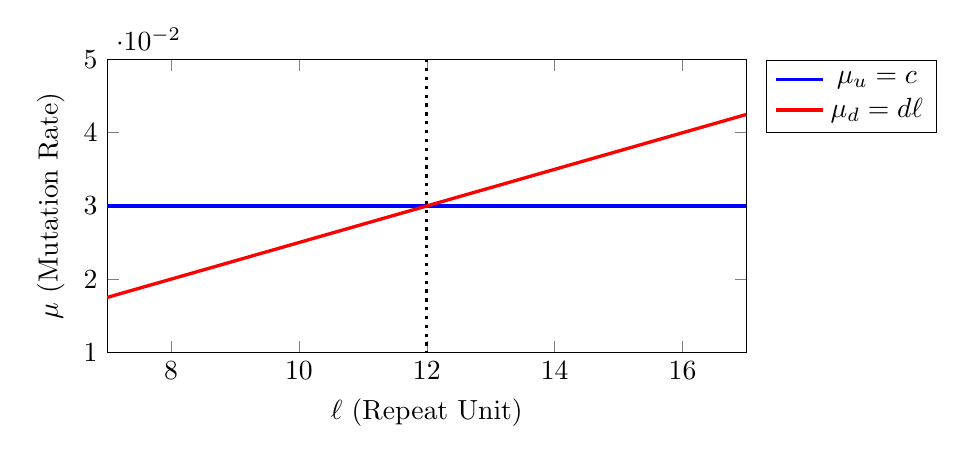
\begin{tikzpicture}
    \begin{axis}[
    width=0.8\linewidth, height=5.3cm,
    ylabel={$\mu$ (Mutation Rate)}, ymin=0.01, ymax=0.05,
    xlabel={$\ell$ (Repeat Unit)}, xmin=7, xmax=17,
    xtick={0, 2, 4, 6, 8, 10, 12, 14, 16, 18, 20, 22, 24, 26},
    samples=100, no markers, legend pos=outer north east, enlargelimits=false,
    domain=0:25
    ]
        \addplot+[very thick]{0.03};
        \addlegendentry{$\mu_u = c$};

        \addplot+[very thick]{0.0025*x};
        \addlegendentry{$\mu_d = d\ell$};

        \addplot+[very thick, black, dotted, forget plot] coordinates {(12, 0) (12, 0.05)};
    \end{axis}
\end{tikzpicture}}
    \caption{Our mutation model for $d=0.0025, c=0.03$.
    Our focal length with these parameters is $\hat{\ell}=12$.}\label{fig:mutationModel}
\end{figure}

%Before building a more complex model, we must first ask, ``When does mutation occur?''.
%Does it occur per generation?
%Per every odd generation?
%The answer to this lies with a quantity known as $\mu \in [0, 1]$, or the \emph{mutation rate}.
%From generation to generation we generate a uniformly distributed random variable between 0 and 1, and ask if this draw
%is below our mutation rate.
%If the answer is yes, we mutate up or down one repeat unit.
%Otherwise, our repeat unit remains unchanged.
%\begin{equation}
%    \begin{cases}
%        \text{mutate} & \mu > \ \sim U(0, 1) \\
%        \text{do not mutate} & \mu \leq \ \sim U(0, 1)
%    \end{cases}
%\end{equation}

\begin{algorithm}[t]
    \SetAlgoLined
    \DontPrintSemicolon
    \Fn{MutateFunction \ {$(c, d, \ell^{(t)})$}} {
        \KwIn{an upward constant mutation bias $c$, downward linear mutation bias $d$, current repeat unit $\ell^{(t)}$}
        \KwOut{a repeat unit from the next generation $\ell^{(t+1)}$}
        $\ell^{(t+1)} \gets \ell^{(t)}$ \;
        \If{$\ell^{(t+1)} = \kappa$}{
            \Return $\ell^{(t+1)}$
        }
        \If{$c < \ \sim U(0, 1)$}{
            $\ell^{(t+1)} \gets \ell^{(t+1)} + 1$ \;
        }
        \If{$d\ell < \ \sim U(0, 1)$}{
            $\ell^{(t+1)} \gets \ell^{(t+1)} - 1$ \;
        }
        \Return $\ell^{(t+1)}$ \;
    }
%    \textbf{end} \;
    \caption{The algorithmic description for $f: \mathbb{M},\mathbb{V} \rightarrow \mathbb{M}$.
    To stay consistent with the definition of $f$ we denote $c$ and $d$ as parameters of the model itself.}
    \label{alg:mutateFunction}
\end{algorithm}

An assumption made with stepwise mutation model is that the probability of mutation is equal for all repeat units.
Ellegren showed that allele unit plays a role in how often mutations
occur~\cite{ellegrenHeterogeneousMutationProcesses2000}.
More specifically, longer repeat units mutate more often than shorter repeat units.
To introduce this repeat unit dependence, we use the following equation:
\begin{equation}\label{eq:linearRepeatUnitDependence}
    \mu = s \cdot \ell
\end{equation}
where $s$ represents the strength of this dependence.
There exists evidence for more complex models such as the exponentially increasing mutation rate of Xu et.\ al.\
~\cite{xuDirectionMicrosatelliteMutations2000}.
In this case, our repeat unit dependence would be represented by:
\begin{equation}
    \mu = s \cdot \exp (\ell)
\end{equation}
Following Sainudiin's general model which included only linear dependence, we made the decision to use the first
equation (\autoref{eq:linearRepeatUnitDependence}).

\section{Presence of Mutational Bias}\label{sec:presenceOfMutationalBias}
There now exists a mutation rate dependence on repeat unit, but the probability of mutating up or down is still
equally likely.
Garza's observed that microsatellites tend to mutate toward a \emph{focal
unit}~\cite{garzaMicrosatelliteAlleleFrequencies1995}.
If the repeat unit of interest $\ell$ is below the focal length at some generation $t$, $\ell$ will have a higher
probability of mutating upward than downward in the following generations.
Conversely if $\ell$ is above the focal length at some generation $t$, $\ell$ will have a higher probability of
mutating downward than upward in the following generations.

Sainudiin's general model uses the functions $\beta : \ell, s \mapsto [0, 1]$ and $\alpha : u, v, \ell \mapsto [0, 1]$
to establish these biases:
\begin{align}
    \beta(\ell, s) &= \mu (1 + (\ell - \kappa)s) \\
    \alpha(u, v, \ell) &= \max (0, \min(1, u - v(\ell - \kappa)))
\end{align}
where $\beta$ is the rate of mutation and $\alpha$ is probability that our repeat unit is incremented (expanded).
Here $u$ represents some constant bias applied toward expansion and $v$ represents the linear bias toward expansion.
A focal unit $\hat{\ell} = ((u - 0.5) / v)$ is specified if we have a greater tendency toward
expansion at lower repeat units ($0.5 < u < 1$) and if the following holds:
$(u - 0.5) / (\Omega - \kappa) < v < \infty$~\cite{sainudiinMicrosatelliteMutationModels2004}.
In other words, a focal unit is defined where the probability of expansion equals the probability of contraction.

\section{Proposed Mutation Model}\label{sec:proposedMutationModel}
This now brings us to our complete mutation model.
To introduce a bias toward some focal unit, we define two mutation rates: the upward mutation rate $\mu_u$ and the
downward mutation rate $\mu_d$.
The total mutation rate is the sum of the two: $\mu = \mu_u + \mu_d$.
We define $\mu_d$ to be dependent on repeat unit, and $\mu_u$ to be constant:
\begin{align}
    \mu_u &= c \\
    \mu_d &= d\ell
\end{align}
where $c$ represents a constant bias for the upward mutation (or, the upward mutation rate itself) and $d$ represents a
linear bias for the downward mutation rate.
We constrain $c > 0, d \geq 0$ to ensure that mutation is always occurring.
The focal unit $\hat{\ell}$ is defined as the intersection between the upward and downward mutation rate, where the
probability of expansion equals to the probability of contraction.
\begin{equation}
    \hat{\ell} = \frac{c}{d}
\end{equation}
This differs from Sainudiin's model usage of $\alpha(u, v, \ell)$, but for our purposes is functionally equivalent and
requires two less parameters.
In addition to the three requirements listed in the previous sections, we constrain that any individuals having repeat
unit $\ell = \kappa$ are unable to mutate back up.
If $f$ is given some repeat unit $\ell$ equal to the lower bound of $\mathbb{M}$, $\ell$ is returned.
This is meant to simulate how microsatellites are lost in populations.

Graphically, this is represented in~\autoref{fig:mutationModel}.
We describe the entire mutation function $f$ in~\autoref{alg:mutateFunction}.
We achieve the first state $\ell^{(t)} + 1$ for some $\ell^{(t)}$ by applying our upward mutation first and saving this
to $\ell^{(t+1)}$.
We achieve states $\ell^{(t)} - 1$ \emph{and} $\ell^{(t)}$ by applying our downward mutation second, after performing
our upward mutation.
Only after performing these two in sequence do we return our mutated repeat unit $\ell^{(t + 1)}$.
